\documentclass[ author={Stephen Livermore-Tozer},
				supervisor={Dr. Peter Flach},
				degree={MEng},
				title={Performing Algorithmic Co-composition Using Machine Learning},
				subtitle={},
				type={research},
				year={2016} ]{dissertation}
				
\usepackage{tikz}
\usetikzlibrary{matrix,chains,positioning,decorations.pathreplacing,arrows}



\begin{document}
	
	\maketitle
	
	\frontmatter
	
	\makedecl
	
	\tableofcontents
	\lstlistoflistings
	
	% -----------------------------------------------------------------------------
	
	\chapter*{Executive Summary}
	
	% Hypothesis
	For my research, I have investigated the hypothesis that existing methods of performing melodic composition using machine learning can be adapted to successfully perform co-composition with a human composer. In this context, success may be measured by subjective impression received from experts in composition. The exact set of tasks involved in the co-composition process is not fixed; part of this research involved finding the tasks that are both a) useful to the composer, and b) within the capabilities of current AI.
	
	The aim of this research project is to attempt to bridge some of the gap between the current theoretical state of algorithmic composition and the practical reality of AI in music.
	
	% Achievements
	In the pursuit of this objective, I have completed the following tasks:
	\begin{itemize}
		\item I surveyed a number of expert composers to identify the tasks within the domain of composition whose partial automation would provide the greatest benefit to the composer.
		\item I performed research over existing machine learning methods for algorithmic composition, determining their applicability and estimated efficacy within the tasks obtained above.
		\item I implemented an application that may be trained on a set of music data (stored in the Midi format) and will provide an attempted continuation of a given musical input, according to the tasks obtained above.
		\item I designed and performed a series of objective and subjective tests to assess the performance of the application and the algorithms that comprise it.
	\end{itemize}
	
	
	% -----------------------------------------------------------------------------
	
	\chapter*{Supporting Technologies}
	
	I used the Anaconda implementation of Python included with the Spyder IDE to create my application. Furthermore, I used a set of libraries implementing utilities and machine learning techniques to create the application. These libraries are: 
	
	\begin{itemize}
		\item Mido for Midi file processing
		\item NumPy for efficient mathematical operations
		\item SciPy for clustering and regression
		\item PyBrain for neural networks
		\item HmmLearn for hidden Markov models
	\end{itemize}
	
	% -----------------------------------------------------------------------------
	
	\chapter*{Acknowledgements}
	
	I would like to thank my supervisor Peter Flach for his guidance over the course of this project in both its technical aspects and in its effective management.
	
	\mainmatter
	
	% -----------------------------------------------------------------------------
	
	\chapter{Contextual Background}
	\label{chap:context}
	
	\section{Overview}
	
	Algorithmic composition is an AI problem concerning the creation of music via some algorithmic process. It is currently one of the topics at the forefront of the greater study of \textit{computational creativity}: the challenge of designing an AI that displays, according to some agreeable definition, creativity. This can be described in another way as algorithmically mimicking various aspects of human intelligence, particularly relating to the conception of novel solutions to problems. The arts are a particular subject of interest for this research, as they are widely considered to be highly creative and distinctly human.
	
	From an AI researcher's perspective, algorithmic composition is not too different in some ways from most other AI tasks: the goal is to design an algorithm that can analyse some complex natural process, derive an abstract model from the available data, and then select actions according to that model. The subject being modelled in this instance however is a psychological process that is both difficult to measure and relatively poorly understood. Many attempts have been made to find an effective way to deal with this problem; some have attempted a bottom-up approach based directly on human psychology, some have attempted to build a top-down model based on known musical principles, and yet others have tried to tackle it as a purely data-oriented task.

	\section{Computational Creativity}
	
	%TODO: Maybe move Machine Learning (ML) to the acronyms section?
	Artificial intelligence as a field has grown a great deal from its first appearance on the academic landscape 60 years ago. It has suffered a fairly shaky history, rising and falling from prominence several times throughout its short life thus far, before reaching its current widespread mainstream adoption and high value in industrial application. Currently techniques that form a part of AI, such as machine learning (ML), are used in a huge number of environments to tackle a wide range of problems. It has become apparent that almost any area in which data analysis plays a large role is a viable target for AI intervention. This not only targets traditional data-heavy fields such as marketing or economics, but also enables complex tasks such as processing natural language, bioinformatics, and autonomous robotic locomotion. While growth and decline is not unknown to AI, it currently occupies a major role in the modern technological landscape and does not show any immediate signs of slowing.
	
	Furthermore, the influence of AI spreads beyond the direct technological applications alone. Even since before the formalization of AI as a field, there has existed a cultural fascination with the concept of intelligent machines. There has been much speculation about the ethical and philosophical implications of the creation of an intelligent mind, and a great deal of fiction has been created with the topic as a central theme. In more recent times as AI has become widely prominent, new hopes and worries have begun to emerge with regards to the social impact, ethical impact, and potential dangers of advanced AI systems. It is in this context that the ultimate capabilities of modern AI technology has fallen into sharp focus.
	
	Currently, the greatest weakness of AI is seen to be in displaying human-like creativity. Although AI is very powerful within domains that have been sufficiently well formalized, there are many fields that remain substantially informal. The most significant of these are the arts. Machines have, to this day, failed to demonstrate any artistic merit of significance that approaches the level of a skilled human. While AI has demonstrated a certain degree of proficiency at specific well-defined tasks within artistic subjects, such as identifying artists from their paintings \cite{blessing2010using} or genres of music \cite{haggblade2011music}, AI remains unable to perform broader creative tasks such as creating or appraising art in a human-like fashion. A good deal of research has been put towards tackling this identified weakness from the academic community, but despite occasional novel results overall progress is proving slow. This deficiency is exacerbated to no small degree by the fact that there is little overlap otherwise between AI and the arts, making it difficult for collaboration or the sharing of knowledge and results between the two.
	
	
	\section{Algorithmic Composition}
	
	One of the areas of artificial creativity currently under focus is algorithmic composition. Algorithmic composition is the general term for the application of algorithms in some form to the task of musical composition - in short, AI that can write music. This is a particularly enticing challenge for those interested in artificial creativity, as music is generally considered to be the most mathematical of all the arts. Various aspects of music at both the physical and compositional level exhibit a very strong degree of structure that can be described mathematically, and conversely elements of mathematics have been directly employed by composers in the creation of their work. This provides a strong argument for music as one of the best suited art forms for analysis by AI, as musical data may be meaningfully digested computationally and consists of patterns and structures that may apparently be learned and predicted. 
	
	%TODO: Give examples of AI-composed music
	In practice however, AI still has a long way to go. Much exploration has been made with the goal of finding an algorithm that produces satisfactory results, but as of yet even the most state of the art musical AIs have clear flaws and limitations. Most ``successful'' AI is specialized for a specific region of composition; common choices include harmonization \cite{freitas2011melody}, jazz improvisation \cite{franklin2001multi}, and full orchestral composition \cite{diaz2011composing}. The best performers within their respective regions produce work that is subjectively assessed as approximately equal to that of a novice composer. Most such work contains noticeable idiosyncrasies however, and despite being able to create amateur-level music the AI consistently fails to produce work comparable with that of skilled composers at even a small probability. This is generally attributed by both artists and certain AI specialists as a lack of creativity; although the AI is skilled at applying certain musical concepts effectively it does not feature the combination of novelty and coherency common to human work. This is not to say that AI as we currently know it is not capable of composition at a human-like level, but that current methods fall short of the mark.
	
	\subsection{Current Challenges}
	
	One of the unique challenges in computational creativity, particularly in algorithmic composition, is that it is very difficult to define creativity to begin with. In some circles of research the goal of computational creativity is in fact to simply understand human creativity in the first place. Because of this, setting an easily measurable objective for the creation of creative AI is implausible if not impossible; instead the metrics used to measure success are typically focused on subjective assessment, either by direct comparison with existing creative work or appraisal by trained art critics. One fairly scientific approach to this is the ``creative Turing test,'' a variant of the traditional Turing test in which a human subject converses through a terminal with both another human and a computer, without being informed which is which. The computer is considered to have passed the Turing test if the subject is unable to distinguish between the human and the computer through the conversation. This translates well into a test of creativity; a human may observe creative works produced by a computer and by a human, and attempt to distinguish which was created by the computer in the same manner. This can be a difficult test to pass depending on the particular creative medium being assessed. One important detail to note with regards to this challenge however is that it does not assess the subjective quality of the piece. This is very understandable given that subjective quality is difficult to define and cannot currently be measured computationally, but it nonetheless is one of the most important factors for any practical application of a creative AI.
	
	Beyond the more abstract difficulties involved however, there are significant technical challenges in replicating human-like musical composition. These include the compositional complexity of most musical pieces (even music considered relatively simple), the colossal variety of styles and genres of music in existence, and the difficulty in obtaining data relating to human appreciation of music. Most AI research thus far has primarily been concerned with creating a robust model for the complex patterns present in real music; typically the goal is either to imitate elements of a pre-specified corpus of music (as in \cite{paiement2007generative} \cite{todd1989connectionist}) or produce wholly original work according to some prior-defined style (\cite{diaz2011composing} \cite{burton1998hybrid} \cite{horowitz1995representing}). 
	
	Despite numerous attempts using a wide range of AI methods (described further in section \ref{sec:abstract-methods}) there have been few significant successes in achieving this goal. The most notable of these is Iamus, a supercomputer running software based on the Melomics system \cite{diaz2011composing}, famous for being the first computer to compose professional contemporary classical music in its own style \cite{scientist2012computer}. Iamus' work has received mixed critical reception, although there is the strong possibility of bias resulting from the fact that composer was already known to be a computer. This system used an evolutionary algorithm with manually-encoded rules as a fitness function (\ref{sec:hybrid-systems}), meaning that it was directly instructed on how to produce classical music without the need for any learning to take place. This design has 
		
	\section{Industrial Impact}
	
	As detailed above, there has been a substantial amount of work invested into algorithmic composition up to this point. It is of notable importance that the vast majority of this work has developed from academic interest only, with very little direct involvement from industry towards the problem (and many of the companies that are involved emerged directly from academia). The cause for this is easily identifiable: there are few current financial incentives to pursue algorithmic composition. Although a high quality artificial composer would certainly be a valuable asset, technology is recognizably quite far away from achieving something effective enough to put to market with a high expected return on investment. This slows down the rate of progress in the study of algorithmic composition, and quite possibly computational creativity as a whole; while current research is going strong, the problem being tackled is immense and the resources available comparatively small. 
	
	The financial incentive for investment in algorithmic composition given the reasonable possibility of achieving success is also quite evident. The music industry is currently valued at over \pounds 10.0 billion globally \cite{smirke2015global}, with the UK retail value worth over \pounds 900 million \cite{riaj2015global}.
	
	%TODO: Tom can probably help you come up with stuff for this section.
	Music as a sector has already been revolutionized by technology in many ways within the past 60 years. The invention of the synthesizer 
	
	\section{Social Impact}
	
	As mentioned above
	
	Additionally, the application of AI to the arts is a heavily romanticized achievement; ``creativity'' is quite universally considered to be a shortcoming of AI, and the creation of art is generally considered to be one of the most significant expressions of human creativity. Because of this, AI that is capable of creating art comparable to that created by humans represents a technological and cultural milestone.
	
	Within the sphere of the arts, music is a key target due to its heavily pattern-based, mathematical nature. Even with these advantages however, AI performance in composition is generally considered to be distinctly poor. According to the majority of subjective measures, AI is identifiably so due to being lacking in creating both interesting short-term melodies and coherent long-term structure. 
	
	
	
	% -----------------------------------------------------------------------------
	
	\chapter{Technical Background}
	\label{chap:technical}
	
	This chapter covers previous work in the field of algorithmic composition, both as a broad overview of the landscape and an in-depth explanation of the particular work directly relevant to this research.

	\section{Abstract Methods for Algorithmic Composition}
	\label{sec:abstract-methods}
	
	Many common types of AI techniques have been used in some way for algorithmic composition. The majority of these techniques can be broadly categorised as one of:
	\begin{itemize}
		\item Knowledge-based models
		\item Supervised learning
		\item Evolutionary algorithms
		\item Hybrid models
	\end{itemize}
	Each of these categories carries their own set of advantages and disadvantages which greatly influence the type of output they produce. Although these categories are not restricted in the type of compositional tasks that they can perform, different techniques may result in completely different uses for the resulting AI. Examples of these different categories, some of the techniques that comprise them, and their strengths and weaknesses follow:
	
	\subsection{Knowledge-Based Models}
	\label{sec:knowledge-systems}
	
	Knowledge-based models use explicitly stored knowledge of some variety to perform computation. They are one of the more intuitive and easy-to-use types of AI, and represent the vast majority of early digital methods for algorithmic composition. There are generally two ways in which this knowledge is obtained; either it is explicitly added by the programmer when the AI is created, or it is learned implicitly from a set of sample cases. The former case has the clear weakness that it can only produce music that it has been explicitly taught how to produce; this puts a harsh limit on the versatility and creativity of the AI. Nonetheless this can be quite an appealing method to use, due to both its computational simplicity and the fact that it can be directly inscribed with compositional principles derived from well-established music theory. Implicitly obtained knowledge on the other hand is much more versatile but is heavily reliant on the quantity and quality of the data provided. The extraction of knowledge from a training set is also a difficult task with many possible solutions - this may also be validly categorised as supervised learning, but is listed here for simplicity's sake. 
	
	%TODO: Find citations for your broad statements, i.e. popularity
	One of the main types of knowledge used in knowledge-based systems is a set of rules/constraints, which is combined with an algorithm that produces an output satisfying these constraints. These techniques are attractive as they have the most direct analogue to music theory. Due to their heavily restricted form however, they are typically poorly suited to performing pure composition. Instead they are typically focused on broad but well-constrained tasks such as harmonization \cite{thomas1985vivace} or jazz improvisation over existing melodies \cite{horowitz1995representing}. Notably in recent decades there has been a significant shift from the use of hard satisfaction of constraints to probabilistic and optimizing methods.
	
	Another common way to store knowledge is as a formal grammar. A formal grammar defines a kind of formal language consisting of a set of symbols that may be arranged according to strict hierarchical structural rules. By creating a grammar that uses musical elements of some kind as its basic symbols, the set of rules used by the grammar can be used to model a style of composition. This is useful when applied to music, due to the natural geometric structure behind most musical composition. However it can also be noted that formal grammars are limited in the degree to which they can comprehend long-term context, an important feature of music that formal grammars struggle to address \cite{moorer1972music}.	 
	
	\subsection{Supervised Learning}
	\label{sec:supervised-learning}
	
	Supervised learning is a subset of machine learning, in which the learning model is trained to approximate some function using a set of clearly defined example inputs and outputs. It is generally applied for tasks involving large-scale data analysis of some kind, such as classifying data samples or identifying relationships between variables in a dataset. It can also be applied to fairly complex decision-based tasks however, as in the case of algorithmic composition. Generally speaking, most supervised learning techniques used for algorithmic composition attempt to model music as a sequential pattern of notes, each associated with some corresponding output depending on the task (such as the subsequent note in melody composition or a harmony in harmonization). This can be considered a specific form of pattern prediction; by understanding the relationship between each set of notes played in a song, you can predict new notes based on a given piece. Due to the popularity and effectiveness of supervised learning in general, it is one of the more popular methods for algorithmic composition.
	
	There are two particular classes of supervised learning techniques that are frequently used in algorithmic composition; the first of these is artificial neural networks (ANNs). ANNs attempt to model the actions of neurons within the human brain in their ability to learn arbitrary mappings between input and output domains. This is very useful for composition as network designs can easily be adapted to different compositional tasks or combined with another techniques (see \ref{sec:hybrid-systems}). The majority of ANNs used in music are recurrent neural networks (RNNs), which have a form of ``memory'' allowing them to model sequences of inputs and understand context. Because of this RNNs are powerful tools for composing short melodies and harmonization. They do however still largely fall short at understanding long-term context and at forming coherent song structure. Additionally as in most ML algorithms, the performance of an ANN is heavily dependent on the musical representation used. Because the inputs to a network are strings of numerical (typically binary) values, the music must be translated into an appropriate format, which the ANN must then learn features from. Because of this a representation in which important features are distinctly visible will heavily outperform one in which those features are more obscured.
		
	The other major class in supervised learning are Markov models. A Markov model is a model representing a stochastic process which transitions through a set of states, where the transition probability is dependent only on the current state (i.e. there is no context or memory). The simplest of these is the Markov chain, which simply acts as a state machine where each state emits a fixed output when arrived at and then probabilistically transitions to another based only on the current state. At first glance this appears to be a crippling weakness, as music is intrinsically involves building on a history of musical events; there are a few ways in which this is resolved. Such methods include \textit{n}-order Markov chains, which have memory of the previous \textit{n} states, or the combination of a Markov chain with other processes. These methods have a limited effectiveness, but still display some stark idiosyncrasies that feel ``out of place'' in a tune. More commonly in recent years however is the use of the hidden Markov model (HMM), in which the exact state of the model at any given time is unknown, and each state outputs values with a certain probability. Training this model involves optimizing both the transition and output probabilities to fit the entire length of the training set, resulting in a much more sophisticated overall model. As a result HMMs see much more use in composition, primarily in non-melodic tasks such as harmonization or rhythm.
	
	\subsection{Evolutionary Algorithms}
	\label{sec:evolutionary-algorithms}
	
	Evolutionary algorithms (EAs) are a relatively recent addition to the algorithmic composition landscape, with the first cases appearing in the early 90s but the majority of practical attempts being made post-2000. EAs are an interesting class of problem solver in that they do not directly solve the problems they are applied to, but instead are a kind of optimization algorithm. One of the keys to an EA is the fitness function it is given; the goal of the EA is to find an optimal input for this function. In the context of music, defining a good fitness function is in itself a very difficult challenge - doing so would mean being able to objectively determine the quality of a musical piece, which is already a major component of the problem of algorithmic composition. Because of this it is quite common to combine EAs with other techniques for use as a fitness function in some capacity. Two of the most common examples of this are training ANNs to act as fitness functions on 
	
	\subsection{Hybrid Systems}
	\label{sec:hybrid-systems}
	
	\section{Artificial Neural Networks in Algorithmic Composition}
	\label{sec:anns}
	
	As described in section \ref{sec:supervised-learning}, artificial neural networks (ANNs) are a powerful class of techniques for approximating functions, and recurrent neural networks (RNNs) extend their functionality to add a form of memory allowing for the comprehension of sequential data. Within this class there have been many different techniques created for performing melodic composition, with many featuring unusual novelties and useful unique properties.
	
	\subsection{Jordan Network With Sparse Pitch Representation and Planning Units}
	
	The first well-documented attempt at using ANNs for musical composition was made by Peter Todd \cite{todd1989connectionist}, who created a simple 3-layered RNN with a topology based on a Jordan network \cite{jordan1997serial} which composed monophonic melodies.
	
	%TODO: Planning units don't strictly work that way, any representation can be used (including real plan values)
	The representation of musical data used by the network is quite basic and has limited scope. The temporal dimension of a song is represented by dividing it into a set of discrete time slices at fixed intervals, and at each of these time slices exactly 1 note may be played or sustained. The input string to the network represents 1 time slice, and consists of a set of values representing pitches, 1 value representing the start of a new note, and a set of values corresponding to ``plans.'' The pitch value for a given time slice is represented simply by taking the pitch of the note $p$ within some user-defined scale (Todd used the C major scale with $p = 0$ for D4 up to $p = 14$ for C6), then setting the $p$-th pitch input to 1 and all others to 0. This only allows a fairly limited range of notes to be played, which reduces the versatility of the network. The value of the ``new note'' input is 1 if a note was started during the time slice, and 0 otherwise. Finally, the ``plan'' inputs have their values set according to the song; there is 1 plan input for each song in the training set, and that input is set to 1 while training with that song (with all other plan inputs set to 0). This input is used by the network to differentiate between the songs that it is trained with, allowing it to behave differently depending on the intended output. Finally, the output of the network is of the same format as the input sans the plan units, and represents the network's estimate for the next time slice.
	
	This particular type of Jordan network is similar to a basic feed forward ANN, with an input layer, a hidden layer, and an output layer, with the input and hidden layers fully connected to the layer ahead. In addition to these connections, two recurrent connections are added: a connection from each $i$-th output neuron to the $i$-th input neuron with weight 1, and a connection from each input neuron to itself (with the exception of the plan neurons) with weight $\alpha < 1.0$ (Todd used $\alpha = 0.7$). This effectively treats the network's output as its input for the next iteration, and causes its inputs to slowly decay instead of disappearing with each iteration. This gives the network an effective memory of recent notes that have been played, with each pitch fading out of memory the longer it goes without being played.
	
	\begin{figure}[!ht]
		\centering
		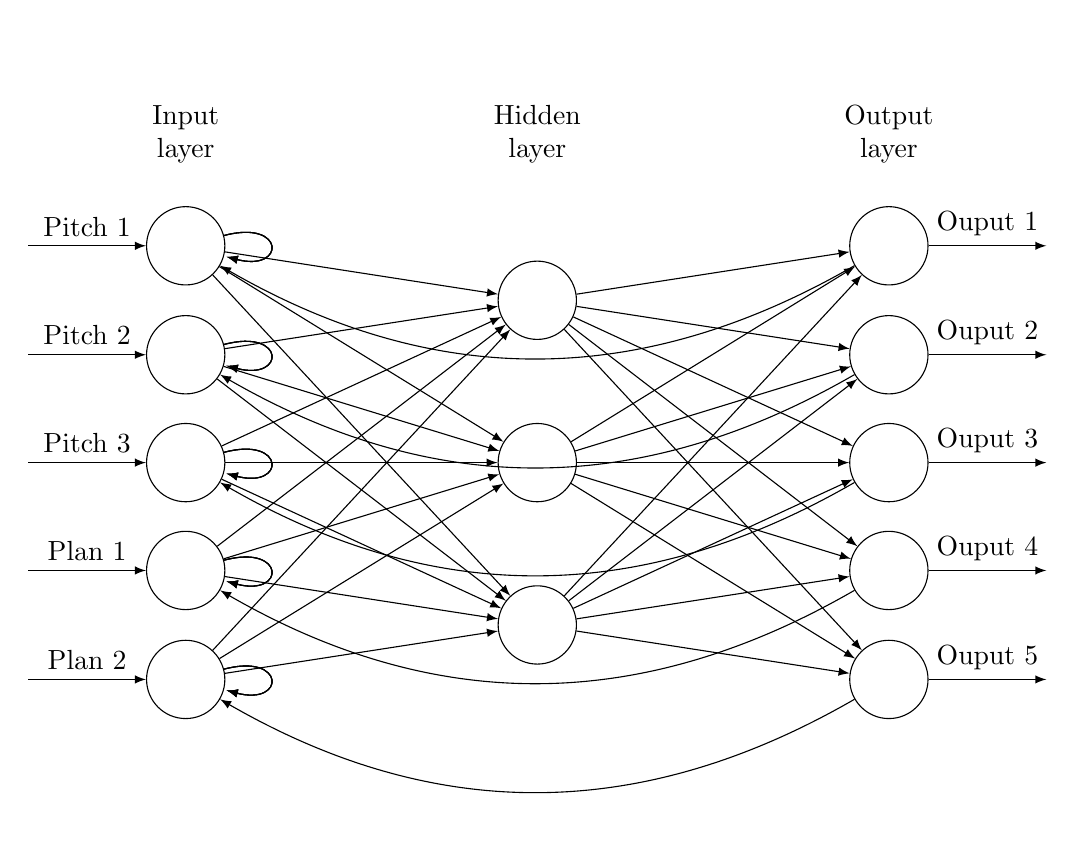
\begin{tikzpicture}[
		plain/.style={
			draw=none,
			fill=none,
		},
		net/.style={
			matrix of nodes,
			nodes={
				draw,
				circle,
				inner sep=10pt
			},
			nodes in empty cells,
			column sep=2cm,
			row sep=-9pt
		},
		>=latex
		]
		\matrix[net] (mat)
		{
			|[plain]| \parbox{1.3cm}{\centering Input\\layer} & |[plain]| \parbox{1.3cm}{\centering Hidden\\layer} & |[plain]| \parbox{1.3cm}{\centering Output\\layer} \\
			& |[plain]| & \\
			|[plain]| & \\
			& |[plain]| & \\
			|[plain]| & |[plain]| \\
			& & \\
			|[plain]| & |[plain]| \\
			& |[plain]| & \\
			|[plain]| & \\
			& |[plain]| & \\
		};
		\foreach \ai [count=\mi ]in {2,4,6}
			\draw[<-] (mat-\ai-1) -- node[above] {Pitch \mi} +(-2cm,0);
		\foreach \ai [count=\mi ]in {8,10}
			\draw[<-] (mat-\ai-1) -- node[above] {Plan \mi} +(-2cm,0);
		\foreach \ai in {2,4,6,8,10}
			{\foreach \aii in {3,6,9}
				\draw[->] (mat-\ai-1) -- (mat-\aii-2);
			}
		\foreach \ai in {2,4,6,8,10}
			{\foreach \aii in {3,6,9}
				\draw[->] (mat-\ai-1) edge[loop right] (mat-\aii-2);
			}
		\foreach \ai in {3,6,9}
			{\foreach \aii in {2,4,6,8,10}
				\draw[->] (mat-\ai-2) -- (mat-\aii-3);
			}
		\foreach \ai [count=\mi ]in {2,4,6,8,10}
			\draw[->] (mat-\ai-3) -- node[above] {Ouput \mi} +(2cm,0);
		\foreach \ai in {2,4,6,8,10}
			\draw[->] (mat-\ai-3) edge[bend left] (mat-\ai-1);
		\end{tikzpicture}
		\caption{An example of a variety of Jordan network}
	\end{figure}
	
	The network is trained using standard backward propagation of errors with gradient descent. The training data is extracted from a set of songs by converting each song to the time slice format as described above, and providing them as input to the network. It is important to note that in traditional operation of the network, the only input to the input layer comes from the recurrent connections from the input layer and the output layer. However this leads to decreased performance during training, due to the fact that the input layer is receiving values from the output layer that are different to the expected output at that stage. Put simply, this means that instead of learning to map each time slice in the training song to the following time slice, the network learns to map the output from its current untrained state to the following time slice in the original song. This problem disappears as the network begins to converge and its actual output begins to match the expected output, but this can take a great deal of time as the training process is essentially chasing a moving target - the network is repeatedly trained to learn an incorrect mapping until it has converged enough to start learning the correct mapping. To overcome this problem, the training process eschews the recurrent connection from the output to input layers and instead directly provides the time slices from the training song as input, allowing the network to start learning the ``real'' mapping immediately.
	
	This network was found to perform reasonably well by Todd. The primary testing metric used in the original paper was the computation required for the network to learn to recreate a number of distinct melodies. The results were fairly promising for the time, with a network of hidden layer size 15 being sufficient to learn up to 4 different songs of 34 time steps each. The number of epochs of training required notably scaled linearly with the number of songs; 2,000 for 1 song, 4,500 for 2 songs, and 8,500 for 4 songs. Reducing the number of hidden units from 15 to 8 however increased the number of epochs required to learn 2 songs to 50,000, due to the increased difficulty of representing the complex patterns of the song with a simpler function.
	
	Following this, a subjective assessment was formed on the ability of the network to create new melodies outside of the training set. This displays one of the advantages of using planning units, as by enabling or disabling different plan inputs the network can be made to output songs of different styles drawing inspiration from one or more of the training songs. A number of observations were made about the original compositions produced by the network: one interesting property it displayed was that when using a single plan unit it tended to output melodies consisting of strings of pitches from the corresponding training melody, but stitched together in new orders at points where the pitches aligned. This ultimately results in the melodies eventually beginning to loop, as at some point the network ends up in a similar state to its initial state and starts playing the opening sequence again. It was also observed to have a very weak understanding of rhythm - the single neuron for representing the start of new notes was insufficiently complex to model the structured nature of musical rhythm. Despite training, the network was unable to establish a relationship between pitch changes and note beginnings.
	
	\subsection{Elman Network with Circle-of-Thirds Pitch}
	
	An alternative simple RNN to the Jordan network as described above is the Elman network \cite{elman1990finding}. The topology of an Elman network is similar to that of a Jordan network, but with different recurrent connections. While in the Jordan network the recurrent feedback is received in the input layer, in the Elman network it is instead received in the hidden layer. 
	
	\section{Distance Modelling with Hidden Markov Models for Monophonic Rhythms }
	
	As discussed in section \ref{sec:supervised-learning}, Markov models tend to have trouble with the kind of complex structure involved in melodic pitch sequences. Using a hidden Markov model helps improve the model's performance in dealing with more complicated sequential patterns. While this type of model is still quite weak in terms of comprehending pitch, it is more capable of recording and recreating simple rhythmic patterns across moderate durations. While this alone is not a common use for HMMs due to their inability to model true long-term patterns, they can be used as part of a hybrid system using a model of rhythmic distances to greater effect \cite{paiement2007generative}.
	
	The HMM used to model rhythmic patterns uses a fairly straightforward representation.	
	
	
%	
%	\section{Overview}
%	
%	There are many different methods for performing algorithmic composition, with a broad range of algorithms and data structures used. Most major AI techniques have many corresponding applications to algorithmic composition - it is also quite common for these techniques to be combined, such as combining neural networks and evolutionary algorithms. % TODO: Link to section
%	Additionally, many of these methods are focused on a specific subtask of composition; popular targets are chord identification, continuation of single line melody, and counterpoint, while many other algorithms focus on more specific tasks (typically relating to a particular genre, such as jazz or baroque).
%	
%	
%	\section{Knowledge-Based Techniques}
%	\label{sec:knowledge-techniques}
%	
%	Knowledge-based systems are those that use a symbolic representation of knowledge to complete a task, and were one of the first forms of AI created. This generally means storing a database of facts and then inferring with this data to resolve statements. In the case of algorithmic composition there are several common abstract approaches that use and represent knowledge in this way. 
%	
%	\subsection{Rule-Based Systems}
%	
%	The first attempts at digital algorithmic composition were knowledge-based, and typically involved encoding explicit, hand-written compositional rules into code and using those rules to create or modify music. These systems notably incorporated no learning of any kind - the behaviour of the program was entirely determined by the initial set of rules and the input (typically a randomly generated melody). This had the effect of making the systems very ``brittle,'' meaning that performance typically dropped dramatically whenever the system encountered an unideal input - a very common occurrence due to the limited scope covered by the initial rules. This can be attributed to the fact that while the compositional principles used by humans are useful and powerful in human hands, they are heavily dependent on the composer providing their own creative input throughout the process.
%	
%	\subsection{Musical Grammars}
%	
%	Other more computationally focused attempts at musical knowledge-based systems have made use of formal grammars. A grammar consists of a set of nonterminal symbols $N$, a set of terminal symbols $\Sigma$ (s.t. $N \cap \sigma = \emptyset$), a start symbol $S \in N$, and a set of production rules that transform strings containing at least 1 nonterminal symbol. A grammar can be used to produce strings by taking a string consisting of the start symbol and repeatedly applying valid production rules to the string until it contains only terminal symbols. Grammars are thus well suited to parsing and generating hierarchical structures recursively, which makes them a good fit for music. 
%	
%	Formal grammars for composition first began to gain popularity in the mid 1970s, with hand-crafted grammars used to represent the structure of music \cite{lidov1973melody}\cite{rader1974method}. 
%	
%	\section{Supervised Learning Techniques}
%	\label{sec:supervised-techniques}
%	
%	Another major branch of work within the field is the use of supervised learning to train AIs through a set of examples, instead of encoding knowledge by hand. This does away with many of the disadvantages of knowledge-based systems, particularly their brittle nature - by learning from examples, the AI can feasibly adapt to work with any particular style of music (with varying difficulty). Currently supervised learning is a very popular method for algorithmic composition, with a majority of papers from the past decade relying on it in some fashion \cite{fernandez2013ai}. This is linked to a combination of the newly widespread availability of musical data to learn from, the increase in computational power (and hence potential complexity of learning models compared to static models), and the high popularity of supervised learning in general.
%	
%	Generally however these methods still have some significant drawbacks. One of the most fundamental of these flaws is the fact that due to their knowledge being entirely derived from a training set they are limited in their ability to develop novel material, instead simply imitating the styles observed during training. There have been attempts to overcome this issue, with many of the most successful attempts using a combination of different techniques (see \ref{sec:hybrid-techniques}).
%	
%	\subsection{Artificial Neural Networks}
%	
%	The most popular class of supervised learning techniques in the context of algorithmic composition are artificial neural networks (ANNs). This can be related to their ability to learn a mapping from one set of data to another, allowing them to be adapted to a complex problem domain such as music. The earliest use of neural networks for algorithmic composition was during the late 80s, where a simple 3-layer recurrent neural network (RNN) was used to compose short monophonic melodies \cite{todd1989connectionist}. Many subsequent ANNs have used a similar design, with adjustments made to the topology and data representation. 
	
	% -----------------------------------------------------------------------------
	
	\chapter{Project Execution}
	\label{chap:execution}
	
%	\section{Objectives}
%	
%	The primary goal of this research is to explore the potential of integrating modern AI methods into the process of human musical composition. Thus it was not only necessary to investigate the AI algorithms themselves, but also their place within a human composer's work environment. The justification for this step is clear - an AI capable of performing or assisting only with tasks that are already trivial adds very little utility. It is therefore necessary as a preliminary step to identify the specific compositional tasks that will receive the greatest positive impact from the introduction of automation.. 
	
	\section{Design}
	
	\subsection{Composition Algorithm}
	
	One of the key details that sets the intended method apart from most other algorithmic composition methods is its purely cooperative nature. This allows for a major performance benefit by offloading a certain portion the work to the human operator. There are three major places in which this offloading can take place: initializing state before generation, guiding the generation process, and adjusting the final generated output. The first is achieved by using the score written by the user as input to create new material from. The third is an intrinsic part of the process, as the final output of the algorithm is provided to the user to be used as they please. The second may be exploited to improve the performance of the algorithm in generating output that is useful or pleasing to the user.
	
	%Out of the wide range of algorithms used in algorithmic composition, the best suited to interactive composition of this variety are evolutionary algorithms (EAs). This is due to their use of a fitness function over a sample population; it is possible to augment the fitness assignment process by allowing the user to provide their preferences as an input to determine each sample's fitness. A number of EAs have been designed with this behaviour in mind in order to overcome the challenge of defining an objective fitness function. This method has the major drawback that it typically causes a large amount of fatigue to the user - providing a rating to each sample once for each generation is a prohibitively large task for a human. To overcome this, it is generally attempted to minimize the population size and number of generations presented to the user, often by querying the user for input over a small subset of fitness evaluations. 
	
	There are a number of ways that this effect could be achieved. One would be the use of evolutionary algorithms. Due to their use of a fitness function to guide their search through the solution space, it is simple and straightforward to integrate user feedback into the EA by using user rating - either as the fitness function, or as some kind of augmentation to the fitness assignment process. A number of EAs have been designed with this behaviour in mind in order to overcome the challenge of defining an objective fitness function. This does however suffer a major drawback in that it is not feasible for an individual user to guide the search process single-handedly; due to the large number of samples that must be judged, user fatigue rapidly becomes a critical constraint. There have been attempts to mitigate this effect through various means, such as reducing the population, number of generations, or novel methods such as using clustering to avoid presenting the user with similar outputs. These methods each present their own limitations however, to an extent that was prohibitive in the case of this research project. 

	% TODO: Explain and justify choice of algorithm									
	
	%\subsection{Musical Fitness}
	%\label{sec:fitness}
	
	%It is accurate to state that the EA is primarily defined by its fitness function: although choice of parameters and initial population may improve the rate at which it approaches an optimal solution, it is the fitness function that defines the optimal solutions. Because of this it is necessary to select a fitness function that will favour good results and prune bad ones. On an objective level this is completely infeasible if not impossible to achieve, hence the need for user intervention to guarantee a good result. Instead a more accurate (if quite abstract) goal for the fitness function should be to minimize the number of bad results presented to the user and adapt well to the user's direction. 
	
	%Through a review of the available literature I have determined that one of the best suited fitness functions to this task is the ARTMAP neural network fitness evaluator \cite{burton1998hybrid}. The main advantages to this method are its ability to adapt to a varied training set, its defined use of user input to direct the search process, and its inherent ability to detect similar patterns - thus preventing the user from being presented with the same results repeatedly. As a supervised learning technique it is necessary to provide a selection of training data
	
	%\section{Population Generation}
	%\label{sec:pop-gen}
	
	%The choice of generation algorithm for the initial population of an EA can have a major impact on that EA's overall performance. An EA with a heuristic that generates a good set of initial solutions can achieve an ideal solution several orders of magnitude faster than an EA that uses a random starting population. This effect is particularly enhanced in scenarios where the output domain is very large while the percentage of good solutions is very small, as is very much the case with musical scores. A simple heuristic for generating approximately feasible melodies does not exist however; in the domain of music finding an approximately good solution is often approximately as difficult as finding a good solution. It is therefore necessary to use an additional algorithmic composition method for the purposes of generating a starting population.
	
	%This method will need to satisfy several requirements to be viable as a population generator:
	
%	\begin{itemize}
%		\item It must have a high run-time speed, as it will need to generate a large number of possible solutions before the EA can begin.
%		\item It must be able to produce many different outputs for the same input, as the population must have variance for the search to be efficient.
%		\item It must be non-interactive in order to not add to the user's fatigue, due to the presence of fatigue as a constraining factor on the EA's performance.
%		\item It must build its solutions off of the score already produced by the user in order for its output to be relevant to the EA.
%	\end{itemize}
	
	%The first requirement implies the use of a technique that uses prior-obtained knowledge to find a solution rather than performing a broader search as with an EA. Two of the most effective and well-documented ways to achieve this are handcrafted knowledge-based systems (\ref{sec:knowledge-techniques}) and supervised learning (\ref{sec:supervised-techniques}). In the former case it is necessary to compose a set of rules and/or constraints that will provide good output for the user's choice of input; this is difficult as these types of techniques are known to be brittle and not very versatile.	In particular most effective rulesets only perform well for specific genres, which prohibits creating a generalist system. Supervised learning on the other hand has the advantage of being versatile and adaptable based on the type of data being worked with. It is also convenient in this case as it is possible to use data already obtained for training the EA's fitness function (\ref{sec:fitness}).
	
	%I reviewed a variety of supervised learning techniques that could be applied effectively to this task. The majority of documented methods use either recurrent neural networks or hidden Markov models trained on a set of melodies. The main advantage of these techniques with regard to composition is that they are effective at extracting features from sequential data consisting of predictable patterns. However, they also tend to be ineffective at representing coherent long-term patterns or understanding non-immediate context, which limits their overall use in composition. Fortunately this shortcoming is partially offset in this scenario by the fact that a skilled human composer will make modifications to the output from this stage as they direct the EA. Because of this it is not necessary for the population generator's output to fully account for certain long-term features, provided that it produces a reasonable variety of good material.
	
	%TODO: Mention use of Gray Code in durations
	
	\subsection{Training}
	
	As discussed in sections \ref{sec:fitness} and \ref{sec:pop-gen}, the AI contains several components using supervised learning. Therefore the results produced by these components, and by extension the AI, will be heavily dependent on the training data provided.
	
	Providing training data for the AI to learn from is potentially a non-trivial task. The reason for this is that the data must fulfil a certain set of constraints, namely:
	
	\begin{itemize}
		\item The data must be stored in a machine-readable format
		\item The input must not contain any features that the AI is not capable of parsing
		\item There must be a strong degree of consistency within the data so that the learned patterns are coherent
	\end{itemize}
	
	The format used to store music throughout this project is the Midi file format \cite{swift1997brief}, which stores music in the form of notes and events instead of sound. This is ideal for this application, as it allows for direct recovery of the exact musical elements contained within each piece of music, a significantly more challenging task when dealing with raw audio. It is also convenient for data acquisition as there exist various large collections of royalty-free midis available to the public. Unfortunately these midis are very often classical music of some variety which often fails to satisfy the second requirement.
	
	The second requirement is one of the most constricting, as for various reasons the AI has many restrictions on the type of musical data it can work with. %TODO: Definitely reference back on this point
	The most harmful of these is the inability to parse or generate polyphonic melodies. This causes some major issues when working with orchestral or piano music due to their frequent use of many melodic lines and chords respectively, which excludes most available classical music. Although it is in some cases possible to isolate a single melodic line, there are quite often no such lines that are both long and substantial enough to be useful for training.
	
	To best overcome these restrictions, the data used was a selection of nursery rhymes transcribed for this research. These have the advantage of being relatively simple and sharing many commonalities such as key and meter, making it much easier for the AI to identify and recreate patterns. They are also universally monophonic due to their vocal nature.
	
	\section{Implementation}
	
		
	\backmatter
	
	\bibliography{dissertation}
	
	\appendix
	
	\chapter{An Example Appendix}
	\label{appx:example}
	
	Content which is not central to, but may enhance the dissertation can be 
	included in one or more appendices; examples include, but are not limited
	to
	
	\begin{itemize}
		\item lengthy mathematical proofs, numerical or graphical results which 
		are summarised in the main body,
		\item sample or example calculations, 
		and
		\item results of user studies or questionnaires.
	\end{itemize}
	
	\noindent
	Note that in line with most research conferences, the marking panel is not
	obliged to read such appendices.
	
	% =============================================================================
	
\end{document}
